\documentclass[12pt]{article}
\usepackage[T1]{fontenc}
\usepackage[utf8]{inputenc}
\usepackage[magyar]{babel}
\usepackage[a4paper,top=0.5in,bottom=0.5in,left=0.5in,right=0.5in,footskip=0.3in,includefoot]{geometry}
\usepackage{amsmath,amsthm,amssymb,amsfonts}
\usepackage{xcolor}
\usepackage[colorlinks,linkcolor=.,citecolor=blue,urlcolor=violet]{hyperref}

% Font related
\usepackage{bbm} % For extended bold and blackboard bold characters
\usepackage{pifont}
%\usepackage{libertine}
\usepackage{lmodern,mathrsfs}

% Graphics related
\usepackage{wrapfig}
\usepackage{graphicx} % Required for inserting images
\usepackage[table,dvipsnames]{xcolor}

% Remark environment
\usepackage[many]{tcolorbox}
\newtcolorbox{remark}[1][]{
	title={\scalebox{1.75}{\raisebox{-.25ex}{\ding{43}}}},
	colframe=white,
	colback=white,
	coltitle=black,
	fontupper=\small,
	sidebyside,
	detach title,
	attach title to upper={\tcblower},
	lefthand width=0.3cm
}

% Macros
\newcommand{\todo}[1]{\textcolor{blue}{TODO: #1}}


\title{SEM18 karóra használati útmutató}
\author{}
\date{\today}

\begin{document}
\frenchspacing
\renewcommand{\abstractname}{\vspace{-\baselineskip}} % To remove the title "abstract"
\maketitle
\begin{abstract}
\end{abstract}

\section{Kezelőszervek jelölése}

\begin{figure}[h!]
\begin{center}
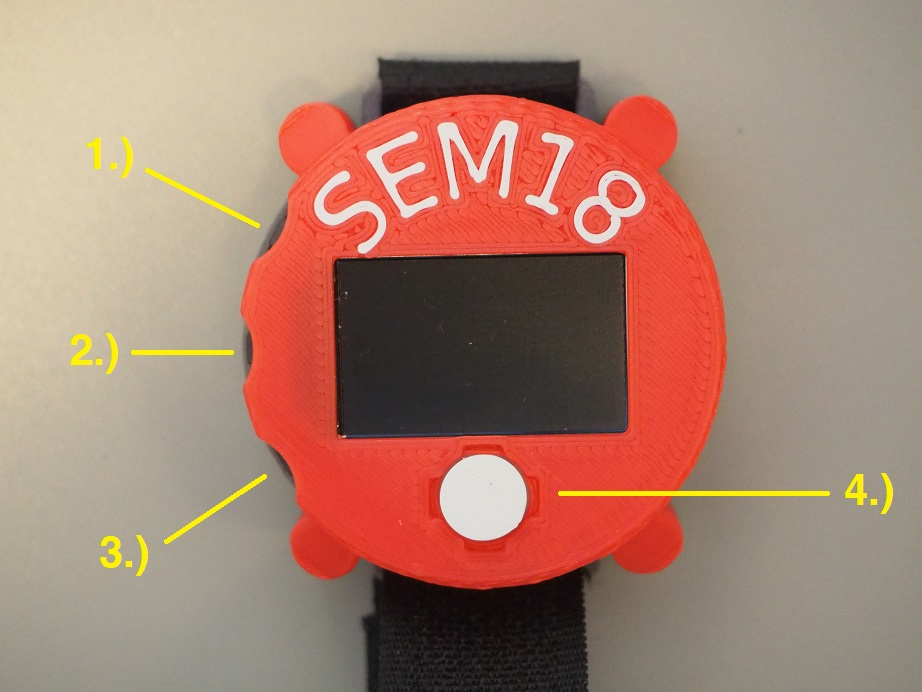
\includegraphics[width=0.6\textwidth]{figures/buttons.jpg}
\end{center}
\label{fig:kezeloszervek}
\caption{Kezelőszervek jelölése a dokumentumban: (1.) felső gomb, (2.) középső gomb, (3.) alsó gomb, (4.) joystick.}
\end{figure}


\section{Óra funkció}
Az óra (jelenleg) két fő funkcióval rendelkezik: óra + dátum kijelzés, és ébresztőóra. A két fő funkció elérése között az alsó gomb megnyomásával lehet váltani. Az óra + dátum kijelzés módban a középső gombbal lehet kikapcsolni a készüléket.

\begin{figure}[h!]
\begin{center}
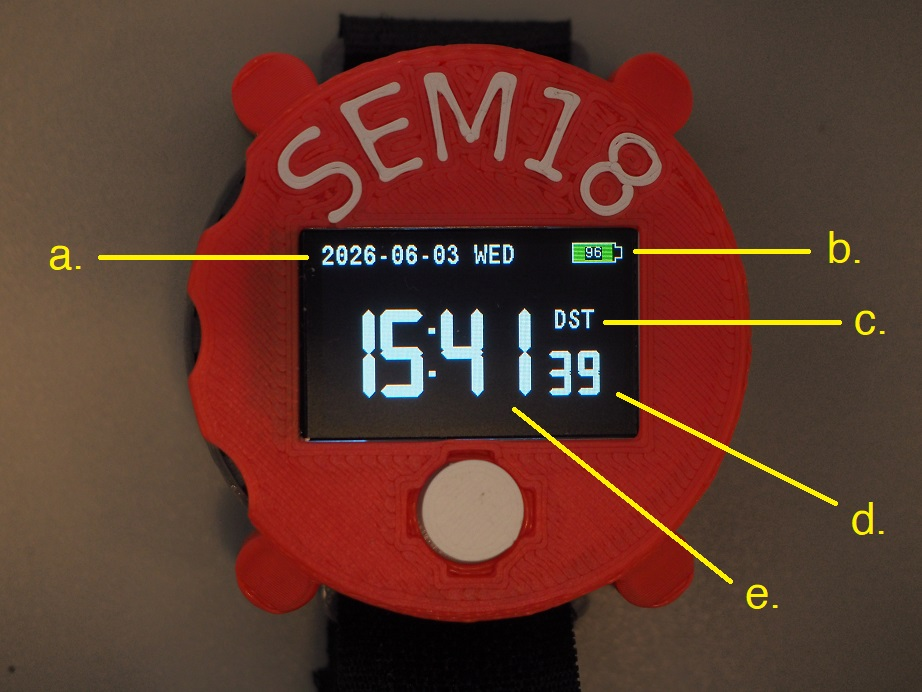
\includegraphics[width=0.6\textwidth]{figures/clock.jpg}
\end{center}
\label{fig:ora}
\caption{Óra kijelzés és részei: (a.) dátum, (b.) akkumulátor töltöttség/feszültség, (c.) nyári időszámítás kijelzés, (d.) másodperc, (e.) óra és perc.}
\end{figure}

Az óra + dátum funkció a valós idejű óra (Real-Time Clock, RTC) periféria által nyilvántartott pillanatnyi időt írja ki a képernyőre. A beállítás a felső gomb hosszú ($>2$~másodperc) megnyomásával kezdeményezhető. A beállítás módban a beállítandó érték villogó megjelenésű, növelése az alsó gombbal, csökkentése a középső gombbal lehetséges. A felső gombbal lehet a következő értékre lépni, ezt rövid hangjelzés is jelzi. A beállítás mód végét egy magasabb frekvenciájú hangjelzés mutatja.

\begin{figure}[h!]
\begin{center}
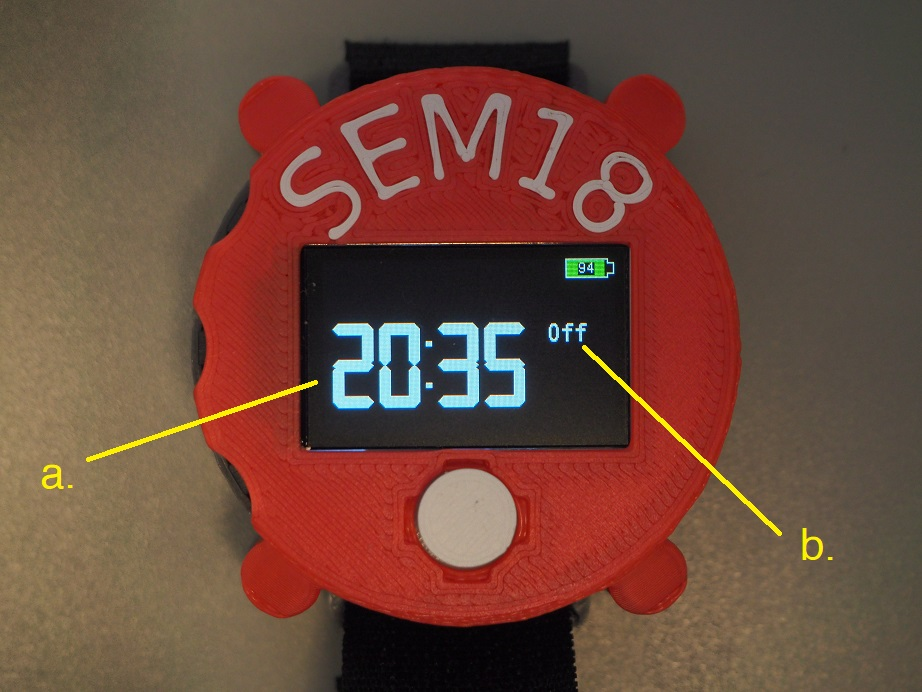
\includegraphics[width=0.6\textwidth]{figures/alarm.jpg}
\end{center}
\label{fig:ebreszto}
\caption{Ébresztési időpont (a.) kijelzése, és (b.) ki/bekapcsolt állapota.}
\end{figure}

Az ébresztő funkció kijelzése \aref{fig:ebreszto}.~ábrán látható. Az ébresztőt a középső gombbal lehet aktiválni, illetve deaktiválni. Az ébresztési időpont beállítása a felső gomb hosszú ($>2$~másodperc) megnyomásával aktiválható, aminek kezelése megegyezik az óra/dátum beállításával.

\begin{remark}
Az ébresztési időpont elérése után az ébresztőóra addig folytatja az ébresztést, amíg bármelyik gomb/joystick irány megnyomásával nem nyugtázzuk.
\end{remark}


\section{Az óra kalibrációja}
Az óra kalibrációjához be kell állítani a pontos időt, és néhány nap/hét múlva megvizsgálni az eltérést egy atomórához képest. Az eltérésből ki kell számolni a hibát ppm-ben. A hiba előjelének (sietés/késés) megfelelő menüpontot kiválasztva beállítható az hiba értéke, amiből a kalibrációhoz szükséges beállításokat a szoftver számolja ki.

\begin{remark}
A kalibráció funkció feltételezi, hogy korábban nem lett beállítva 0-tól eltérő hiba. Amennyiben mégis be lett állítva, akkor annak ppm hibáját hozzá kell adni a számított hibaértékhez. A hibaérték az első feszültség alá helyezéskor nullázódik.
\end{remark}


\section{Tetris}
A játék a joystickkel játszható, de el kell hozzá forgatni az órát $90^\circ$-kal. Kilépés a középső gomb megnyomásával lehetséges.

\section{Snake}
A játék a joystickkel játszható, kilépés a középső gomb megnyomásával lehetséges.

\section{Szoftverfrissítés}
A szoftver kétféleképpen frissíthető:
\begin{enumerate}
\item Dedikált programozóval (pl. ST-Link, CMSIS-DAP, J-Link, stb.) a NYÁK-on elhelyezett programozó csatlakozón át,
\item Beépített bootloader használatával USB-n keresztül.
\end{enumerate}

A bootloader aktiválásához reset közben nyomni kell a felső gombot. A bootloaderből kilépés történhet a reset gomb megnyomásával, vagy a PC oldali program is képes elindítani a letöltött programot.

\begin{remark}
Bizonyos példányoknál (de nem mindegyiknél) a bekapcsolás is resetnek számít, tehát a felső gombot nyomva bekapcsoláskor a bootloader kezd futni.
\end{remark}

A szoftver bootloaderen keresztül az STM32CubeProgrammer segítségével frissíthető.

%\begin{wrapfigure}{r}{0.6\textwidth}
%	\vspace{-0.5cm}
%	\begin{center}
%		\includegraphics[width=0.58\textwidth]{figures/nvic.jpg}
%	\end{center}
%	\label{fig:nvic}
%	\caption{Megszakításvezérlő (NVIC) a processzor mellett.}
%\end{wrapfigure}

%\begin{remark}
%A kivételkezelők definíciói megtalálhatók a processzormag dokumentációjában, ami Cortex-M0 processzor esetében itt található: \url{https://developer.arm.com/documentation/dui0497/a/the-cortex-m0-processor/exception-model/exception-types}
%\end{remark}


\end{document}
